\documentclass{article}
\usepackage{graphicx}
\usepackage[dvipsnames,table]{xcolor}
\usepackage[utf8]{inputenc}
\usepackage{siunitx}
\usepackage[american,siunitx]{circuitikz}
\usepackage{amsmath}
\usepackage{svg}
\usepackage{booktabs}
\usepackage{float}
\usepackage{xparse, xfp}
\usepackage{multirow}
\usepackage{tikz}
\usepackage{karnaugh-map}
\usepackage{pdfpages}
\usepackage{hyperref}
\hypersetup{
    colorlinks=true,
    linkcolor=blue,
    filecolor=magenta,      
    urlcolor=cyan,
}
\usepackage{caption} 
\captionsetup[table]{skip=10pt}

\usetikzlibrary{calc}
%\usepackage[landscape]{geometry}
\renewcommand{\thesubsection}{\thesection.\alph{subsection}}
\newcommand{\equal}{=}
\newcommand{\greyrule}{\arrayrulecolor{black!30}\midrule\arrayrulecolor{black}}
\makeatletter
\newcommand\currcoor{\the\tikz@lastxsaved,\the\tikz@lastysaved}
\makeatother
\newcolumntype{:}{@{\hskip\tabcolsep\color{black!30}\vrule\hskip\tabcolsep}}

\ExplSyntaxOn
\NewExpandableDocumentCommand \groupify { O{\,\allowbreak} m m }
  { \jakob_groupify:nnn {#1} {#2} {#3} }
\cs_new:Npn \jakob_groupify:nnn #1 #2 #3
  { \__jakob_groupify_loop:nnw { 1 } {#2} #3 \q_recursion_tail {#1} \q_recursion_stop }
\cs_new:Npn \__jakob_groupify_loop:nnw #1 #2 #3
  {
    \quark_if_recursion_tail_stop:n {#3}
    \exp_not:n {#3}
    \int_compare:nNnTF {#1} = {#2}
      { \__jakob_groupify_sep:n }
      { \exp_args:Nf \__jakob_groupify_loop:nnw { \int_eval:n { #1+1 } } }
          {#2}
  }
\cs_new:Npn \__jakob_groupify_sep:n #1 #2 \q_recursion_tail #3
  {
    \tl_if_empty:nF {#2} { \exp_not:n {#3} }
    \__jakob_groupify_loop:nnw { 1 } {#1}
    #2 \q_recursion_tail {#3}
  }
\ExplSyntaxOff

\title{ECE 2200L\\Introduction to Microelectronics Circuits Laboratory\\\,\\Experiment 6\\Bipolar Junction Transistor Biasing Circuits and Bias Point Stability\\\,\\Report}
\author{Choi Tim Antony Yung}
\date{October 21, 2020}
\begin{document}
\maketitle

\thispagestyle{empty}
\setcounter{page}{0}

\newpage

\section*{Objective}

To study and experiment on three types of DC biasing circuits for BJTs, and compare the stability of the bias point in these circuits.
\section*{Prelab}
\begin{figure}[H]
  \centering
  \begin{circuitikz}
    \draw
    node[npn](npn){}
    (npn.C) node[circ]{} node[right]{C} to [R,l_=\SI{1.5}{\kilo\ohm}, i<=$I_C$] ++(0,2) coordinate(vcc) node[vcc]{\SI{10}{\volt}}
    (vcc) -- ++(-2,0) to[R=\SI{470}{\kilo\ohm}] (\currcoor|-npn.B) to[short, i>=$I_B$] (npn.B) node[circ]{} node[above]{B} 
    (npn.E) node[circ]{} node[right]{E} node[ground]{}
    ;
  \end{circuitikz}
  \caption{Circuit 1}
  \label{fig:ckt1}
\end{figure}

Assuming $V_{BE}=\SI{0.7}{\volt}$
\begin{align}\label{eqn:ckt1}
  I_B    &= \frac{10-0.7}{470000} =\SI{19.8}{\micro\ampere}\\
  I_C    &= \beta I_B             = \beta\SI{19.8}{\micro\ampere}\\
  V_{CE} &= 10-1500\beta I_B          = 10-1500\beta\left(19.8\times10^{-6}\right)\SI{}{\volt}
\end{align}

\begin{table}[H]
  \caption{Quiescent point parameter of circuit 1 for transistor with different $\beta$}
  \centering
    \begin{tabular}{rrrr}
      \toprule
       &$Q_1$&$Q_2$&\% difference\\
      \midrule
      $\beta$&100&124&$24\%$\\
      $I_B$&\SI{19.8}{\micro\ampere}&\SI{19.8}{\micro\ampere}&$0\%$\\
      $I_C$&\SI{1.98}{\milli\ampere}&\SI{2.46}{\milli\ampere}&$24\%$\\
      $V_{CE}$&\SI{7.03}{\volt}&\SI{6.32}{\volt}&$-10\%$\\
    \bottomrule
  \end{tabular}
  \label{tab:ckt1}%
\end{table}


\newpage
\begin{figure}[H]
  \centering
  \begin{circuitikz}
    \draw
    node[npn](npn){}
    (npn.C) node[circ]{} node[right]{C} to [R,l_=\SI{510}{\ohm}, i<=$I_C$] ++(0,2) coordinate(vcc) node[vcc]{\SI{10}{\volt}}
    (vcc) -- ++(-2,0) to[R=\SI{220}{\kilo\ohm}] (\currcoor|-npn.B) to[short, i>=$I_B$] (npn.B) node[circ]{} node[above]{B}
    (npn.E) node[circ]{} node[right]{E} to[R,l_=\SI{510}{\ohm}] ++(0,-2) node[ground]{}
    ;
  \end{circuitikz}
  \caption{Circuit 2}
  \label{fig:ckt2}
\end{figure}

Assuming $V_{BE}=\SI{0.7}{\volt}$
\begin{align}\label{eqn:ckt2}
  I_E    &= (1+\beta)I_B\\
  \SI{10}{\volt} &= 220000I_B+0.7+510(1+\beta)I_B\\
  I_B    &=\frac{9.3}{220510+510\beta}\\
  I_C    &= \beta I_B = \frac{9.3\beta}{220510+510\beta}\\
  V_{CE} &= \left(10-\frac{(510)(9.3)\beta}{220510+510\beta}\right)-\frac{510(1+\beta)9.3}{220510+510\beta}
\end{align}

\begin{table}[H]
  \caption{Quiescent point parameters of circuit 2 for transistors with different $\beta$}
  \centering
    \begin{tabular}{rrrr}
      \toprule
       &$Q_1$&$Q_2$&\% difference\\
      \midrule
      $\beta$&100&124&$24\%$\\
      $I_B$&\SI{34.3}{\micro\ampere}&\SI{32.8}{\micro\ampere}&$-4\%$\\
      $I_C$&\SI{3.43}{\milli\ampere}&\SI{4.06}{\milli\ampere}&$18\%$\\
      $V_{CE}$&\SI{6.49}{\volt}&\SI{5.84}{\volt}&$-10\%$\\
    \bottomrule
  \end{tabular}
  \label{tab:ckt2}%
\end{table}

\newpage
\begin{figure}[H]
  \centering
  \begin{circuitikz}
    \draw
    node[npn](npn){}
    (npn.C) node[circ]{} node[right]{C} to [R,l_=\SI{820}{\ohm}, i<=$I_C$] ++(0,2) coordinate(vcc) node[vcc]{\SI{10}{\volt}}
    (vcc) -- ++(-2,0) to[R=\SI{15}{\kilo\ohm}] (\currcoor|-npn.B) coordinate(npnB) to[short, i>=$I_B$] (npn.B)  node[circ]{} node[above]{B}
    (npn.E) node[circ]{} node[right]{E} to[R=\SI{220}{\ohm}] ++(0,-2) node[ground](gnd){}
    (npnB) to[R=\SI{3.3}{\kilo\ohm}] (\currcoor |- gnd) -- (gnd)
    ;
  \end{circuitikz}
  \caption{Circuit 3}
  \label{fig:ckt3}
\end{figure}

Assuming $V_{BE}=\SI{0.7}{\volt}$
\begin{align}\label{eqn:ckt3}
  I_B    &= \frac{10-V_B}{15000}-\frac{V_B}{3300} = \frac{20190-18300V_E}{49500000} \\
  I_E    &= (1+\beta)I_B = \frac{(1+\beta)(20190-18300V_E)}{49500000} = \frac{V_E}{220}\\
  V_E    &= \frac{44418000(1+\beta)}{53526000+4026000\beta}\\
  I_B    &= \frac{20190-18300\frac{44418000(1+\beta)}{53526000+4026000\beta}}{49500000}\\
  I_C    &= \beta I_B\\
  V_{CE} &= V_C-V_E= (10 - 820I_C)-V_E
\end{align}

\begin{table}[H]
  \caption{Quiescent point parameters of circuit 3 for transistors with different $\beta$}
  \centering
    \begin{tabular}{rrrr}
      \toprule
       &$Q_1$&$Q_2$&\% difference\\
      \midrule
      $\beta$&100&124&$24\%$\\
      $I_B$&\SI{44.3}{\micro\ampere}&\SI{36.5}{\micro\ampere}&$-17\%$\\
      $I_C$&\SI{4.42}{\milli\ampere}&\SI{4.53}{\milli\ampere}&$2\%$\\
      $V_{CE}$&\SI{5.39}{\volt}&\SI{5.28}{\volt}&$-2\%$\\
    \bottomrule
  \end{tabular}
  \label{tab:ckt3}%
\end{table}

\section*{Result}
\subsection*{Circuit 1}
The following is the experimental data obtained from circuit 1.

\begin{table}[H]
  \caption{$V_B$, $V_C$ and $V_E$ of circuit 1 for transistor with different $\beta$}
  \centering
    \begin{tabular}{rrrr}
      \toprule
       &$Q_1$&$Q_2$&\% difference\\
      \midrule
      $\beta$&100&124&$24\%$\\
      $V_B$&\SI{0.642}{\volt}&\SI{0.644}{\volt}&$0\%$\\
      $V_C$&\SI{5.984}{\volt}&\SI{5.552}{\volt}&$-7\%$\\
      $V_E$&\SI{0}{\volt}&\SI{0}{\volt}&$0\%$\\
    \bottomrule
  \end{tabular}
  \label{tab:ckt1_exp}%
\end{table}

$I_B$, $I_C$ and $V_{BE}$ can be derived from the below equations,
\begin{align}\label{eqn:ckt1_2}
  I_B    &= \frac{10-V_B}{470000}\\
  I_C    &= \beta I_B\\
  V_{CE} &= V_C-V_E
\end{align}

\begin{table}[H]
  \caption{Quiescent point parameter of circuit 1 for transistor with different $\beta$}
  \centering
    \begin{tabular}{rrrr}
      \toprule
       &$Q_1$&$Q_2$&\% difference\\
      \midrule
      $\beta$&100&124&$24\%$\\
      $I_B$&\SI{19.9}{\micro\ampere}&\SI{19.9}{\micro\ampere}&$0\%$\\
      $I_C$&\SI{1.99}{\milli\ampere}&\SI{2.47}{\milli\ampere}&$24\%$\\
      $V_{CE}$&\SI{5.984}{\volt}&\SI{5.552}{\volt}&$-7\%$\\
    \bottomrule
  \end{tabular}
  \label{tab:ckt1_calc}%
\end{table}

\newpage

\subsection*{Circuit 2}
The following is the experimental data obtained from circuit 2.

\begin{table}[H]
  \caption{$V_B$, $V_C$ and $V_E$ of circuit 1 for transistor with different $\beta$}
  \centering
    \begin{tabular}{rrrr}
      \toprule
       &$Q_1$&$Q_2$&\% difference\\
      \midrule
      $\beta$&100&124&$24\%$\\
      $V_B$&\SI{2.91 }{\volt}&\SI{3.086}{\volt}&$0\%$\\
      $V_C$&\SI{7.74 }{\volt}&\SI{7.56 }{\volt}&$-7\%$\\
      $V_E$&\SI{2.296}{\volt}&\SI{2.467}{\volt}&$0\%$\\
    \bottomrule
  \end{tabular}
  \label{tab:ckt2_exp}%
\end{table}

$I_B$, $I_C$ and $V_{BE}$ can be derived from the below equations,
\begin{align}\label{eqn:ckt2_2}
  I_B    &= \frac{10-V_B}{220000}\\
  I_C    &= \beta I_B\\
  V_{CE} &= V_C-V_E
\end{align}

\begin{table}[H]
  \caption{Quiescent point parameter of circuit 2 for transistor with different $\beta$}
  \centering
    \begin{tabular}{rrrr}
      \toprule
       &$Q_1$&$Q_2$&\% difference\\
      \midrule
      $\beta$&100&124&$24\%$\\
      $I_B$&\SI{32.2}{\micro\ampere}&\SI{31.4}{\micro\ampere}&$0\%$\\
      $I_C$&\SI{3.22}{\milli\ampere}&\SI{3.89}{\milli\ampere}&$20\%$\\
      $V_{CE}$&\SI{5.444}{\volt}&\SI{5.093}{\volt}&$-6\%$\\
    \bottomrule
  \end{tabular}
  \label{tab:ckt2_calc}%
\end{table}

\newpage

\subsection*{Circuit 3}
The following is the experimental data obtained from circuit 3.

\begin{table}[H]
  \caption{$V_B$, $V_C$ and $V_E$ of circuit 3 for transistor with different $\beta$}
  \centering
    \begin{tabular}{rrrr}
      \toprule
       &$Q_1$&$Q_2$&\% difference\\
      \midrule
      $\beta$&100&124&$24\%$\\
      $V_B$&\SI{1.731}{\volt}&\SI{1.738}{\volt}&$0\%$\\
      $V_C$&\SI{6.031}{\volt}&\SI{6.008}{\volt}&$0\%$\\
      $V_E$&\SI{1.08 }{\volt}&\SI{1.083}{\volt}&$0\%$\\
    \bottomrule
  \end{tabular}
  \label{tab:ckt3_exp}%
\end{table}

$I_B$, $I_C$ and $V_{BE}$ can be derived from the below equations,
\begin{align}\label{eqn:ckt3_2}
  I_B    &= \frac{I_C}{\beta}\\
  I_C    &= \frac{10-V_C}{820}\\
  V_{CE} &= V_C-V_E
\end{align}

\begin{table}[H]
  \caption{Quiescent point parameter of circuit 3 for transistor with different $\beta$}
  \centering
    \begin{tabular}{rrrr}
      \toprule
       &$Q_1$&$Q_2$&\% difference\\
      \midrule
      $\beta$&100&124&$24\%$\\
      $I_B$&\SI{48.4}{\micro\ampere}&\SI{39.3}{\micro\ampere}&$-18\%$\\
      $I_C$&\SI{4.84}{\milli\ampere}&\SI{4.87}{\milli\ampere}&$1\%$\\
      $V_{CE}$&\SI{4.951}{\volt}&\SI{4.925}{\volt}&$-1\%$\\
    \bottomrule
  \end{tabular}
  \label{tab:ckt3_calc}%
\end{table}

\newpage

\subsection*{Circuit 4}

\begin{figure}[H]
  \centering
  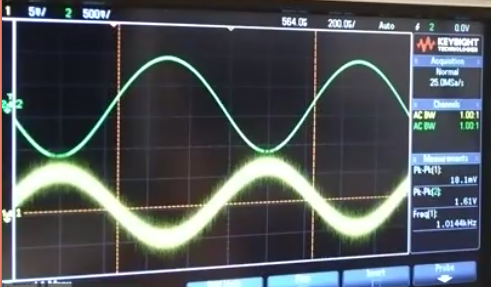
\includegraphics[width=\textwidth]{ECE2200L_Lab6.png}
  \caption{Oscilloscope output for circuit 4}
  \label{fig:scope}
\end{figure}

Gain = $\frac{\SI{1.61}{\volt}}{\SI{18.1}{\milli\volt}}=89$

\section*{Conclusion}
As demonstrated in this document above, circuit \ref{fig:ckt3} setup is considerably stable across transistors with different $\beta$ value compare to circuit \ref{fig:ckt1} and circuit \ref{fig:ckt2}
\end{document}
